\documentclass[manuscript,anonymous,review]{acmart}

% ---------------------------------------------------------------
% MEASUREMENT-PAPER REFRAME of the UniKV work.
% The TACO mechanism paper lives in ../UNIKV-TACO/main.tex and is
% unchanged. This version reframes the same evidence: the instrument
% is UniKV, the contribution is what it measured.
% Venue formatting (IISWC/IEEEtran, MLSys, CAL) is a later step; we
% keep acmart here so it builds with the existing toolchain.
% ---------------------------------------------------------------
\acmJournal{TACO}
\acmYear{2026}
\setcopyright{acmlicensed}
\citestyle{acmnumeric}

\usepackage{microtype}
\usepackage{subcaption}

\begin{document}

\title{What Vanishing Transfer Cost Does Not Buy: Measuring Exact
       KV-Cache Retention on Unified Memory}

\author{Alp Demir Ekinci}
\affiliation{%
  \institution{Sabanc\i{} University}
  \city{Istanbul}
  \country{T\"urkiye}}
\email{alp.ekinci@sabanciuniv.edu}
\renewcommand{\shortauthors}{Ekinci}

% ---------------------------------------------------------------
% ABSTRACT — findings-forward, as the genre expects
% ---------------------------------------------------------------
\begin{abstract}
Unified-memory accelerators remove the explicit CPU--GPU transfer that
KV-cache offloading systems are designed around, which suggests that on
such hardware a cache should never discard anything: spill it to the
shared pool and recall it exactly. We built that policy into
\texttt{llama.cpp} on an Apple M4~Pro and measured what it costs. It
costs more than the transfer model predicts, for reasons the transfer
model cannot express.

We report five findings. First, the cost of exact retention is
\emph{affine and dominated by a fixed term}: entering the two-tier
attention path costs $9.0$\,ms per decode step regardless of how much
is retained, against $3.1\,\mu$s per retained cell. Moving the tier
onto the accelerator over the same physical pages removes $69\%$ of the
fixed term --- and $24.5$--$30.5\%$ of the per-cell term depending on
the estimator, over identical physical pages, so on unified memory even
the data cost depends on which processor reads it and cannot be derived
from a byte count. The reduction is not
free: a device-visible tier is charged against the working set at
capacity, trading the bounded device footprint that motivated the
design. Second, \emph{retrieval does not distinguish
lossless retention from heavy-hitter eviction}: an H2O evictor
implemented in the same fork recovers a mid-context passkey at the same cache
budget and the same number of demotions, while running faster; what
lossless retention uniquely provides is token-identical reproduction of
the no-eviction computation, held over $512$ generated tokens on two
prompts where the evictor diverges within the first $16$, and for which
the evictor runs $11.4\%$ faster
where three-fifths of the context is non-resident and $1.3\%$ faster
where one-fifth is. Third, \emph{transfer cost
cannot be simulated by delay injection alone} --- asynchronous
dispatch largely absorbs an undrained delay. At the one coefficient
measured under both conditions, draining costs $0.713 \pm 0.068$\,tok/s
($t = 10.5$) while the injected delay itself is undetectable
($t = 0.11$). The drain has no separable price of its own: it costs
nothing at $\alpha = 0$ in two independent blocks and $0.981 \pm
0.247$\,tok/s at $\alpha = 1$, so it cannot be calibrated away, and
delay injection and the instrument that exposes it are one mechanism
rather than two additive costs. Fourth, \emph{capacity limits appear
at execution, not allocation}: contexts allocate and generate at
$1.80\times$ the advisory Metal working-set budget and then fail when
the memory is touched, so allocation-only probing finds no limit where
one exists. The per-token device cost that sets the ceiling is
$136$--$194$\,KiB rather than the $128$\,KiB of KV, governed by the
micro-batch --- a parameter usually tuned for throughput --- which
moves the ceiling by $1.7\times$. Fifth, \emph{rolling-window context shift is more expensive
than heavy-hitter eviction}, because it re-encodes rotary position
embeddings across the whole cache while the evictor drops cells.

We report the measurement protocol that these results required --- a
thermally randomised block design, per-arm verification of kernel
settings from run logs, and an isochronal design that decorrelates
retained-set size from device temperature --- because on a passively
cooled accelerator the naive versions of these experiments produce
confident wrong answers.
\end{abstract}

\begin{CCSXML}
<ccs2012>
   <concept>
       <concept_id>10010520.10010521.10010537</concept_id>
       <concept_desc>Computer systems organization~Architectures</concept_desc>
       <concept_significance>500</concept_significance>
   </concept>
   <concept>
       <concept_id>10010583.10010786.10010813</concept_id>
       <concept_desc>Hardware~Memory and dense storage</concept_desc>
       <concept_significance>300</concept_significance>
   </concept>
</ccs2012>
\end{CCSXML}

\ccsdesc[500]{Computer systems organization~Architectures}
\ccsdesc[300]{Hardware~Memory and dense storage}

\keywords{KV cache, LLM inference, unified memory, workload
characterization, measurement methodology, Apple Silicon}

\maketitle

% ---------------------------------------------------------------
\section{Introduction}
\label{sec:intro}

The key-value cache dominates memory pressure in long-context language
model inference, and the literature that manages it divides cleanly by
an assumption about hardware. Fixed-budget eviction methods --- H2O,
Scissorhands, SnapKV, NACL, Ada-KV~\cite{zhang2023h2o,liu2023scissorhands,li2024snapkv,chen2024nacl,feng2025adakv}
--- assume only on-device memory is usable and ask which tokens to
discard. Offloading methods --- FlexGen, InfiniGen, ShadowKV, and
others~\cite{sheng2023flexgen,lee2024infinigen,sun2025shadowkv,cheng2025lmcache}
--- assume evicted state can live in host memory but that moving it
back is expensive, and design around that cost.

Unified-memory hardware appears to dissolve the second assumption, and
it is worth separating two things the term covers. On Apple Silicon,
CPU and GPU address one physical DRAM pool~\cite{apple2024m4pro,mlx2024}:
demotion moves no bytes, because there is nowhere to move them to.
NVIDIA Grace Hopper instead offers coherent addressing across
NVLink-C2C~\cite{nvidia2024gh200}, where a remote access is
transparent but still crosses an interconnect --- transfer shrinks
rather than vanishing. This paper measures the first case only, on a
single physical pool, which is the setting in which the argument below
is strongest and where our findings therefore apply. Whether they
carry to a coherent-interconnect machine is an open question we cannot
answer with the hardware we have, and Section~\ref{sec:threats} says
which of them we expect to survive the move.

In the shared-pool case, if moving KV state between tiers is nearly
free, the apparent implication is that a cache on such hardware should
never discard anything: demote it to the shared pool and recall it
exactly, so that a full cache becomes a routine event rather than a
terminating error.

We implemented that policy and measured it. The implication does not
survive contact with the hardware, and the reasons are the contribution
of this paper. Removing the transfer does not make exact retention
cheap, because the cost that remains is not proportional to what is
retained --- it is a fixed per-step price for leaving the
accelerator's fused attention path. And exactness turns out to buy less
than expected against a heavy-hitter evictor, which recovers the same
information more cheaply while producing a different computation.

\paragraph{Findings.} We report five, each self-contained in
Sections~\ref{sec:f1}--\ref{sec:f5}:

\begin{enumerate}
  \item The per-step cost of exact retention is affine in both
    configurations we measured, $31.317\,\text{ms} + 3.099\,\mu\text{s}
    \cdot n_\text{spill}$ with the tier read by the host and
    $25.252\,\text{ms} + 2.153\,\mu\text{s} \cdot n_\text{spill}$ with
    it read by the accelerator. Both terms fall, including the data
    term that a byte count alone would hold fixed, and the reduction
    costs the bounded device footprint (Section~\ref{sec:f1}).
  \item Retrieval does not separate lossless retention from
    fixed-budget eviction. An H2O heavy-hitter evictor, implemented
    inside the same fork so that it shares the harness, the cache
    layout and the measurement path, recovers a
    mid-context passkey at the same budget and is faster; only
    token-identity with the no-eviction reference separates them ---
    exact over $512$ generated tokens on two prompts against divergence
    within the first $16$ --- and the evictor runs $11.4\%$ faster at
    $C = 1024$ and $1.3\%$ faster at $C = 2048$ (Section~\ref{sec:f2}).
  \item Simulated transfer cost is dominated by the instrumentation
    used to expose it. At the one coefficient measured under both
    conditions the drain costs $0.713 \pm 0.068$\,tok/s ($t = 10.5$)
    while the injected delay is undetectable ($t = 0.11$). The drain's
    cost is not a constant that can be subtracted off: it is zero at
    $\alpha = 0$ and grows with the delay it exposes
    (Section~\ref{sec:f3}).
  \item Capacity limits appear at execution rather than allocation.
    Contexts allocate and run at $1.80\times$ the advisory working-set
    budget, then fail with a refused command buffer when the memory is
    touched. Device cost per token is $136$--$194$\,KiB rather than the
    $128$\,KiB of KV, set by the micro-batch, which moves the ceiling
    by $1.7\times$ (Section~\ref{sec:f4}).
  \item Rolling-window context shift is more expensive than
    heavy-hitter eviction, by $7.7\%$ at $C = 1024$, because it
    re-encodes RoPE across the whole cache
    (Section~\ref{sec:f5}).
\end{enumerate}

\paragraph{Scope.} This is a characterization study on one accelerator,
one model, and one runtime. We are explicit throughout about which
findings are properties of the hardware, which of the runtime, and
which of our own implementation, because those three carry very
different generality. Section~\ref{sec:threats} collects the threats to
validity rather than distributing them.

% ---------------------------------------------------------------
\section{Background and Instrument}
\label{sec:background}

\subsection{KV caching and the two policy families}

Autoregressive decoding caches the key and value tensors of every
previous token so that each new token attends over them without
recomputation. The cache grows linearly with sequence length, layers,
and batch size, and it is the dominant memory consumer in long-context
serving~\cite{kwon2023vllm}. Table~\ref{tab:families} summarises how
existing policies respond and where the policy we instrument sits.

\begin{table}[t]
  \centering
  \caption{KV-cache policy families and the regime each assumes.
  $\alpha$ denotes the normalised cost of moving KV state between
  tiers; the last column records where attention over non-resident KV
  executes.}
  \label{tab:families}
  \renewcommand{\arraystretch}{1.25}
  \begin{tabular}{@{}p{0.20\columnwidth}p{0.28\columnwidth}p{0.11\columnwidth}p{0.20\columnwidth}p{0.10\columnwidth}@{}}
    \toprule
    \textbf{Family} & \textbf{Representative systems} & \textbf{Regime}
      & \textbf{Overflow response} & \textbf{Attn.} \\
    \midrule
    Fixed-budget eviction
      & H2O, Scissorhands, SnapKV, NACL, Ada-KV
      & $\alpha \rightarrow \infty$
      & lossy discard or compression
      & device \\
    Transfer-aware offloading
      & FlexGen, InfiniGen, ShadowKV, TailorKV, SpeCache, LMCache
      & large finite $\alpha$
      & spill with managed or hidden recall traffic
      & device \\
    Attention offloading
      & FastDecode, vLLM CPU swap
      & large finite $\alpha$
      & exact spill; compute migrates instead of data
      & host \\
    \midrule
    Exact retention (instrumented here)
      & ---
      & $\alpha \approx 0$
      & exact spill and exact recall
      & host \\
    \bottomrule
  \end{tabular}
\end{table}

\subsection{The instrument}
\label{sec:instrument}

Our measurements come from a modified \texttt{llama.cpp} in which four
cache policies are branches of one binary, selected by the environment
variable \texttt{UNIKV\_POLICY}. Because the policies share a binary,
model, prompts, seed, batch tiling, and thermal protocol, a policy
comparison is a single-variable relaunch:

\begin{itemize}
  \item \textbf{Policy 0}, upstream: return an error when the cache is
    full, ending generation.
  \item \textbf{Policy 1}, rolling window: evict the oldest token and
    shift surviving positions down. This is the mechanism upstream
    ships as \texttt{-{}-context-shift}~\cite{llamacpp_contextshift},
    whose principled form is the attention-sink window of
    StreamingLLM~\cite{xiao2024streamingllm}; a sink parameter selects
    between the naive and sink-preserving variants.
  \item \textbf{Policy 3}, exact retention: on overflow, copy the
    oldest resident cells' keys and values to a host-side store keyed
    by (layer, token position), preserving absolute positions, and free
    the resident cells. Attention then ranges over the union of both
    tiers --- query--key scores computed separately against resident
    and spilled cells, concatenated, and reduced under a
    \emph{single} softmax, with the spilled-tier matrix multiplications
    pinned to the CPU backend so host-resident KV is never copied to
    the device. The result is numerically equal to attending over the
    full retained context while the device holds only $C$ cells. The
    fused flash-attention kernel cannot ingest an externally staged
    tier, so this path requires it disabled.
  \item \textbf{Policy 4}, H2O: accumulate per-token attention mass
    across all queries; at overflow retain the most recent half of the
    budget plus the highest-mass tokens among the
    rest~\cite{zhang2023h2o}. Eviction removes cells without shifting
    positions, so RoPE stays exact for survivors.
\end{itemize}

Two auxiliary gates support the experiments: \texttt{UNIKV\_ALPHA}
prices a simulated inter-tier transfer (Section~\ref{sec:f3}), and
\texttt{UNIKV\_DRAIN} decouples the pipeline drain from that
coefficient. A per-\texttt{decode()} CSV records cache occupancy, the
spilled-set size, and a demotion flag.

\subsection{Platform}

An Apple M4~Pro with 24\,GB of unified LPDDR5 memory and Metal~3,
running Llama~3.1~8B Instruct quantised to Q4\_K\_M, all 32
transformer layers plus the output layer offloaded to the GPU, built
from upstream commit \texttt{9725a313b}. The runtime reports a Metal
\texttt{recommendedMaxWorkingSetSize} of $17179.89$\,MB --- a decimal-MB
rendering of a $16$\,GiB budget, i.e.\ $16384$\,MiB, which is the unit
every footprint in this paper is expressed in. Per-token KV
size is $128$\,KiB ($32 \times 8 \times 128 \times 2 \times 2$ bytes),
which we confirm against the runtime's own memory breakdown.

% ---------------------------------------------------------------
\section{Measurement Methodology}
\label{sec:method}

On a passively cooled accelerator the naive form of every experiment
below produces a confident wrong answer. We describe the protocol
first because it is a precondition for the findings, and because the
failure modes generalise to any thermally unconstrained device.

\paragraph{The thermal problem.} This device droops ${\approx}21\%$
over a few minutes of sustained load: within a single position-balanced
block we observe throughput ranging from $39.9$ to $31.6$\,tok/s from
heat alone. That is an order of magnitude larger than most effects we
wish to resolve. Worse, it is time-correlated, so any experiment whose
independent variable is swept in order aliases temperature onto the
variable. A monotonic $\alpha$ sweep on this device can manufacture, or
mask, a trend larger than the effect itself.

\paragraph{Randomised block with cooldowns.} Every comparison in this
paper runs as a randomised block: all arms are shuffled under a
recorded seed, a fixed $200$\,s cooldown precedes every run, and each
arm is repeated across trials with the per-arm mean reported. This
holds per-arm standard deviations to $0.01$--$0.41$\,tok/s where the
uncooled thermal swing is $8.2$\,tok/s.

\paragraph{Setting verification from run logs.} Kernel and tiling
settings are parsed back out of each run's own log rather than trusted
from harness source, and a comparison fails if they differ across arms.
This is not paranoia: an early version of one comparison in this work
drew its arms from two harnesses that disagreed on flash attention
(one enabled, one disabled) and on batch tiling ($256$ against $512$),
which would have folded a separately measured $12.4\%$ kernel penalty
into a policy result. The check is cheap and it caught a real error.

\paragraph{Isochronal design for size-dependent costs.}
Section~\ref{sec:f1} measures cost against retained-set size. The
obvious experiment --- one long decode run, plotting per-step cost
against $n_\text{spill}$ --- cannot work here, because
$n_\text{spill}$ grows monotonically with elapsed time and so does
temperature: they are the same variable, and no within-run regression
separates them. A single long run gives an apparent slope of
$5.32\,\mu$s per cell; a constant-work thermal control run
(policy 1, window pinned, nothing spilled) shows $+6.0$\,ms of droop
over $303$\,s, and subtracting it linearly gives $4.18\,\mu$s. Both are
contaminated. We therefore establish the spilled tier to a target size
during \emph{prefill} and then time a short decode burst, so
$n_\text{spill}$ is fixed before the measurement rather than growing
through it. Targets are run in randomised-block order with cooldowns.

\paragraph{Instrumentation is not free.} Setting the per-step CSV log
causes the runtime to synchronise at both ends of every
\texttt{decode()} call, draining the pipeline on every step. Throughput
comparisons in this paper therefore run \emph{uninstrumented}, and we
use the log only where the quantity of interest is a count rather than
a rate.

\paragraph{The units the runtime prints are not the units it reports
footprints in.} The cheapest error in this paper to make and the
hardest to see. Metal advertises its budget through
\texttt{recommendedMaxWorkingSetSize}, which the runtime prints in
decimal megabytes --- $17179.89$\,MB --- while every allocation figure
in the same log, including the memory-breakdown rows we compare against
it, is in binary mebibytes. The two scales differ by $1.048576$, so
dividing a MiB footprint by the printed MB budget understates the
result by $4.9\%$. We made exactly that error, and it survived into a
draft table, an abstract and a headroom calculation before an
independent check caught it, because every affected number was
plausible: a ratio of $0.64$ where the truth was $0.67$ reads as a
comfortable margin either way, and $1.72$ against $1.80$ still supports
the same claim. Nothing in the arithmetic is difficult. What makes it
dangerous is that the error is multiplicative and small enough to
preserve every qualitative conclusion, so no result looks wrong. The
defence is to convert once, at the point of parsing, and to state the
unit in the column heading of every table that carries a footprint.

\paragraph{Throttling is processor-dependent, and counterbalancing does
not save you.} The most expensive methodological lesson here came from
trying to avoid the cooled protocol. Comparing our two spill
configurations with a counterbalanced A/B --- alternating them within a
session rather than running a cooled block --- gave answers that were
wrong in \emph{both} directions: it overstated the device-visible
speedup, $+46.5\%$ against a cooled $+25.9\%$, and understated the cost
of exactness against H2O, $+7.8\%$ against a cooled $+11.4\%$.

The cause is that the arms load different processors and therefore
throttle at different rates. Across one session the CPU-pinned arm
drifted $-23\%$ while the accelerator-side arms moved $-6\%$ and
$-10\%$; every arm improves on a cool machine, but that arm improves
most. Counterbalancing defends against \emph{order} effects within a
session. It does nothing about an arm being differentially sensitive to
the session's thermal level, which biases the mean rather than the
ordering, so the bias survives averaging and points in whichever
direction the comparison happens to face.

Two consequences worth stating plainly. Where compared configurations
place work on different processors, only a cooled block produces
trustworthy magnitudes. And a more careful design was more wrong than a
less careful one: our original single-shot measurement of the speedup
($+24\%$) landed closer to the cooled value than the counterbalanced
A/B did. That is not an argument for single shots --- it is a reminder
that the A/B's error was systematic rather than random, and increasing
$n$ does not touch systematic error.

\paragraph{Migrate the whole subgraph or none of it.} A related trap
sits in the implementation rather than the protocol. Moving the spilled
tier onto the accelerator requires releasing two backend pins, not the
one obvious from the data flow. Releasing only the first is
\emph{worse} than releasing neither --- $22.9$ against $30.4$\,tok/s in
smoke measurement --- because the graph then half-migrates, with the
score product on the accelerator and the value product still pinned,
and the scheduler inserts dozens of splits that copy a multi-megabyte
permuted view every step. An experimenter who removes the obvious pin,
measures, and finds a regression would reasonably conclude the approach
does not work. It does; it is partial migration that does not.

\paragraph{Artifacts.} All CSVs, per-run logs, and analysis files are
provided as supplementary material, with each headline number traceable
to the run block that produced it.

% ---------------------------------------------------------------
\section{Finding 1: Both Cost Terms Depend on Which Processor Reads
         the Tier}
\label{sec:f1}

\paragraph{What we measured.} Per-step decode cost as a function of the
number of cells held in the spilled tier, at $C = 1024$ with flash
attention off, under the isochronal design of
Section~\ref{sec:method}, in two configurations of the same
implementation. In the first the spilled tier lives in a host
allocation and its matrix multiplications are pinned to the CPU
backend. In the second the tier is allocated from the resident cache's
own Metal buffer type --- genuinely zero-copy on this hardware --- and
the pins are removed, so the accelerator attends over both tiers.

\begin{figure}[t]
  \centering
  
\includegraphics[width=0.55\columnwidth]{fig5_recall_cost}
  \caption{Per-step decode cost against spilled-set size at
  $C = 1024$, for a tier read by the host and by the accelerator. Both
  are affine; the shaded wedge between the fits is the difference,
  widening from $6.14$\,ms at $n_\text{spill} = 0$ to $13.89$\,ms at
  $8192$. The intercept gap is the removable handoff cost, $69\%$ of
  the fixed term; the widening is the per-cell term falling $30.5\%$ on
  these mean-based fits, over identical physical pages and therefore
  identical byte counts.}
  \label{fig:recall}
\end{figure}

\paragraph{Result.} Figure~\ref{fig:recall} plots both series. Each is
affine over the measured range, and both fits are tight:
\begin{align}
\label{eq:recall-cost}
t^{\text{cpu}}_\text{step} &\approx 31.317\,\text{ms}
  + 3.099\,\mu\text{s} \cdot n_\text{spill}, \\
\label{eq:recall-cost-dev}
t^{\text{dev}}_\text{step} &\approx 25.252\,\text{ms}
  + 2.153\,\mu\text{s} \cdot n_\text{spill},
\end{align}
with slope standard errors $0.0764$ and $0.0055$ and residual standard
deviations $0.832$ and $0.059$\,ms. The regressor is the
\emph{measured} spilled-set size, which exceeds the harness's target by
a constant $79.5$ cells in every run; fitting against the target
instead shifts each intercept upward by that offset times the slope and
leaves the slopes unchanged. Subtracting each arm's own no-spill mean
($22.554$ and $22.544$\,ms, statistically indistinguishable at
$t = -0.28$, so the tier is genuinely inert when unused) gives fixed
terms of $\gamma^{\text{cpu}} = 8.763$\,ms and
$\gamma^{\text{dev}} = 2.708$\,ms, a $69\%$ reduction. The two slopes
are separable at $t = 12.34$, a per-cell reduction of $30.5\%$.
As a further control, $\gamma^{\text{cpu}}$ reproduces across nights
and a rebuilt binary.

\paragraph{How well-determined the per-cell result is.} The $30.5\%$
figure is estimator-dependent and we report the sensitivity rather than
the better number. Refitting the identical runs on per-burst medians
instead of means gives $2.853$ against $2.155\,\mu$s per cell, a
reduction of $24.5\%$. Essentially all of the movement is in one arm:
the device-visible slope shifts by $0.08\%$ while the CPU-pinned slope
falls $7.9\%$.

The reason is a dispersion asymmetry that is itself worth reporting. At
the largest target the CPU-pinned bursts have within-burst step
standard deviations of $3.39$--$6.03$\,ms and mean-minus-median gaps of
$+1.26$ to $+3.16$\,ms; the device-visible bursts have $0.14$--$0.20$\,ms
and $+0.03$\,ms. One arm's per-step distribution carries a heavy right
tail that the other does not, and a mean-based fit charges that tail
entirely to the per-cell term. Host-side attention does not merely cost
more per step, it costs more \emph{variably}, and the conceptual claim
below rests on the conservative estimate of $24.5\%$ rather than on
$30.5\%$.

\paragraph{Why it matters.} The fixed term is a handoff cost and it is
removable. Entering the two-tier path costs $9.0$\,ms per step when
the spilled matmuls run on the host, paid in full as soon as a single
cell has spilled, and $2.9$\,ms when they run on the accelerator over
the same physical pages. That confirms the obvious hypothesis: most of
what looked like the price of retention was the price of leaving the
fused path.

The per-cell term is the result we did not expect, and the expectation
was ours rather than the literature's. When we wrote our own cost
model, $\delta$ was the \emph{data} term --- the cost of streaming
bytes, and therefore independent of which processor streams them, since
on unified memory they are the same bytes in the same DRAM. We are not
aware of a published model that states processor-independence in this
form, and we do not claim to refute one; the offloading systems of
Table~\ref{tab:families} price transfer across a real interconnect,
where the question does not arise. What we can offer is the
quantification: on this machine, moving the tier from host to
accelerator over identical physical pages makes each retained cell
$24.5$--$30.5\%$ cheaper depending on the estimator. A model that
prices retention as bytes times a constant, as ours did, will be wrong
by that much on unified memory, and the practical consequence is that
the data term has to be measured per placement rather than derived from
a byte count.

Two mechanisms could produce that gap and our measurements do not
separate them. The GPU may sustain more bandwidth to the same pages
than the CPU does, or the two attention kernels may differ in how
efficiently they consume what they read --- Metal threadgroup
scheduling against host SIMD over the same data. Distinguishing them
needs an achieved-bandwidth measurement on both paths, which we did not
take, so ``the GPU reads these pages faster'' should be read as one
candidate rather than a conclusion. A third possibility can be
excluded from the geometry: this model's KV cells are $128$\,KiB, which
is exactly $\text{f16}$ at $32$ layers, $8$ KV heads and head dimension
$128$, so the spilled entries are unquantized on both paths and no
dequantization step distinguishes them. The weight quantization plays
no part in the recall path.

\paragraph{The catch, and it is the whole trade.} Making the tier
device-visible costs the property that motivated the design. A host
allocation is invisible to the Metal working set: with the tier pinned
to the CPU, free device memory is unchanged at every spill capacity we
tried, and a $16$\,GiB tier runs. Allocated from a device buffer type
the tier is charged in full, at \emph{capacity} rather than occupancy,
so device memory becomes $O(C) + O(\text{spill capacity})$ and the
configuration acquires a ceiling --- measured at $81\,920$--$90\,112$
cells in Section~\ref{sec:f4}. Exact retention therefore offers two
operating points and not one: bounded device memory at $9$\,ms of
fixed cost per step, or $2.9$\,ms at a device footprint that grows with
what you retain. There is no configuration that gives both, and which
one is on the table is a decision the system designer has to make
rather than a default to inherit.

\paragraph{Validity boundary.} Neither
Equation~(\ref{eq:recall-cost}) nor
Equation~(\ref{eq:recall-cost-dev}) may be extrapolated. At
$n_\text{spill} = 61\,471$, in the capacity run of
Section~\ref{sec:f4}, the CPU-pinned per-step cost is $666$\,ms where
Equation~(\ref{eq:recall-cost}) predicts $222$\,ms, exceeding the
prediction by $200\%$. The affine
form describes the regime we measured ($n_\text{spill} \lesssim 10^4$),
not a scaling law.

The isochronal design also self-heats, since larger targets need longer
prefills immediately before the timed burst, and the two arms are not
equally exposed: at the largest target the CPU-pinned bursts run
$93.5$--$95.0$\,s against $44.8$--$46.9$\,s device-visible, on a device
that droops measurably under sustained load
(Section~\ref{sec:method}). Residual heating therefore inflates
$\delta^{\text{cpu}}$ more than $\delta^{\text{dev}}$, which means the
measured gap between them \emph{overstates} the true one. Both per-cell
terms are upper bounds, and so is their difference: $30.5\%$, or
$24.5\%$ on medians, should be read as a ceiling on the effect rather
than an estimate of it. Settling this needs a constant-work thermal
control per arm at each target, matched on burst duration rather than
step count --- the analogue of the control used in
Section~\ref{sec:method} --- which we have not run.

% ---------------------------------------------------------------
\section{Finding 2: Retrieval Does Not Separate Retention from Eviction}
\label{sec:f2}

\paragraph{What we measured.} Whether a policy recovers a fact stated
early in a long prompt, and whether it reproduces the continuation that
an unconstrained cache would have produced. A five-digit passkey is
stated at token position ${\approx}\,219$ of a 3834-token prompt,
followed by filler and a closing question. Six arms, one harness, one
run block, \texttt{-b 256 -ub 256}, flash attention off on all six and
verified per arm from run logs, greedy decoding at fixed seed.

\begin{table}[t]
  \centering
  \caption{Passkey retrieval; $n = 1$ per arm over a 32-token
  continuation. Greedy decoding at a fixed seed is deterministic, so
  the arms are exactly reproducible but carry no variance estimate, and
  every equivalence in \emph{this} table is established only to that
  horizon; Table~\ref{tab:horizon} extends the retention and H2O arms
  to $512$ tokens on two prompts. All four
  $C = 1024$ arms take the same
  42 demotions at the same $128$\,MiB device budget. Retrieval does not
  separate the policies; reproducing the reference computation does.
  DWR is the distinct-word ratio of the continuation, a coherence
  proxy.}
  \label{tab:quality}
  \renewcommand{\arraystretch}{1.25}
  \begin{tabular}{@{}llcccl@{}}
    \toprule
    \textbf{Policy} & \textbf{Cache} & \textbf{Demot.} & \textbf{DWR} &
      \textbf{Passkey} & \textbf{Output vs.\ ref.} \\
    \midrule
    No-eviction reference & $C = 4096$ &  0 & $0.818$ & retrieved & --- \\
    Exact retention, idle & $C = 4096$ &  0 & $0.818$ & retrieved & token-identical \\
    Exact retention       & $C = 1024$ & 42 & $0.818$ & retrieved & token-identical \\
    H2O                   & $C = 1024$ & 42 & $0.667$ & retrieved & diverges \\
    StreamingLLM ($k{=}4$)& $C = 1024$ & 42 & $0.321$ & lost      & diverges \\
    Naive rolling window  & $C = 1024$ & 42 & $0.125$ & lost      & diverges \\
    \bottomrule
  \end{tabular}
\end{table}

\paragraph{Result.} Table~\ref{tab:quality} reports the six arms. H2O
retrieves the passkey. Both window policies
lose it. Exact retention retrieves it and additionally reproduces the
reference continuation at the level of sampled token IDs, which H2O
does not: H2O emits ``\ldots(The pass key is 48291.)\ The pass key is
48291'' where the reference emits ``\ldots(Note: The pass key is
repeated many times in the text, but it is''. This six-arm survey runs
to a 32-token continuation, short enough that an evicting policy could
agree by luck, so we extend the two arms that carry the claim
separately.

\paragraph{How far the identity extends.} A second block, run to $512$
generated tokens on two prompts, tests the arms whose behaviour the
recommendation rests on: the no-eviction reference, exact retention
with the tier CPU-pinned, exact retention with it device-visible, and
H2O, all at $C = 1024$ against a $3834$-token prompt. The same
discipline applies --- one block, \texttt{-b 256 -ub 256}, flash
attention off and parsed back from each run's own log, greedy at fixed
seed, EOS suppressed so every arm generates the full budget. The
second prompt is deliberately unlike the first: the published probe is
low-entropy filler, which may be unusually easy to reproduce, so we
added a $3834$-token prefix of a technical README, matched to the same
token count, in which the model generates markdown structure, URLs and
repository names rather than recycling its own input.

\begin{table}[t]
  \centering
  \caption{First divergence from the no-eviction reference over $512$
  generated tokens, $C = 1024$, two prompts. Greedy decoding at a fixed
  seed is deterministic, so $n = 1$ per cell. Identity is
  whole-sequence rather than prefix agreement: the reference and both
  retention arms share a single checksum over all $512$ sampled IDs on
  each prompt. The control is the reference at the smaller cache, which
  fills at exactly $262$ generated tokens
  ($3834 + 262 = 4096$).}
  \label{tab:horizon}
  \renewcommand{\arraystretch}{1.25}
  \begin{tabular}{@{}llll@{}}
    \toprule
    \textbf{Arm} & \textbf{Tier} & \textbf{Passkey} & \textbf{Prose} \\
    \midrule
    Exact retention & CPU-pinned     & none in $512$ & none in $512$ \\
    Exact retention & device-visible & none in $512$ & none in $512$ \\
    H2O             & ---            & token $16$    & token $0$ \\
    \midrule
    \emph{Control:} reference at $C = 4096$ & --- & none in $262$ & none in $262$ \\
    \bottomrule
  \end{tabular}
\end{table}

Table~\ref{tab:horizon} reports it. Both retention arms reproduce the
reference exactly for all $512$ tokens on both prompts; H2O diverges
within the first $16$ tokens on both. The comparison is not vacuous:
each retention arm ends the run with $3321$ cells in the spilled tier
against $1024$ resident, so roughly three-quarters of the working set
is non-resident and the identical output is being produced across
$3321$ spill-and-recall round trips, while H2O evicts the same $3321$
cells and the reference logs no demotion at all. The device-visible
tier matches the CPU-pinned tier exactly, which is what makes the
placement decision priced in Section~\ref{sec:f1} a free choice on
this evidence rather than a quality trade.

The reference here runs at $C = 8192$ rather than the $4096$ used for
the 32-token survey, because $3834 + 512$ cells no longer fit and a
$C = 4096$ reference would itself evict. The control row establishes
that the substitution is free: the reference at $C = 4096$ agrees with
the reference at $C = 8192$ over every token it produces before its
cache fills, so the reference does not depend on the cache size.

Continuing past the first mismatch turned out to matter, because the
two prompts fail differently in a way the divergence index hides. On
the passkey probe H2O diverges once and never recovers, falling into a
repetition loop and sitting at $3.1\%$ agreement --- coincidence level
--- for the remaining $384$ tokens. On prose it decoheres gradually
instead, agreeing with the reference on $64.1\%$, $37.5\%$, $21.9\%$
and $7.8\%$ of tokens in successive $128$-token windows: both arms are
generating the same \emph{kind} of thing, a list of language bindings,
so they keep colliding on boilerplate while the contents drift apart.
The two divergence indices, $16$ and $0$, are single observations and
we do not treat the exact values as stable; what the data support is
that H2O diverges within the first $16$ tokens on both prompts, and
earlier on the harder one.

One thing this block does not show is H2O failing the task. It
recovers the planted key on the passkey prompt and opens its
continuation with it, as it does at the 32-token horizon. The claim is
narrow by construction: exact retention reproduces the reference token
stream and H2O does not.

\paragraph{Why H2O succeeds.} The passkey is a rare, high-information
token in repetitive filler, so it accumulates attention mass well above
the filler median long before the closing question is seen. In the
survivor trace it ranks second and fourth in the entire cache, behind
only the position-0 attention sink, which outweighs the next token by
two orders of magnitude. H2O's known weakness --- it must decide what
matters before seeing the query --- is not exercised by this prompt. A
probe whose needle goes unattended until the question arrives would
likely separate the policies; we did not run one, and we would present
it as a targeted stress test rather than a headline, because a probe
chosen to make a comparator fail is not evidence about the general
case.

\paragraph{The comparator is not a strawman.} Three checks. At
$C = 4096$ with no overflow, policy 4 emits a token-identical sequence
to stock, so the scoring machinery does not perturb the computation. It
beats the naive window at the same budget, our pre-registered sanity
condition. And its survivor set is $512$ recent cells plus $511$ heavy
hitters, $231$ of them drawn from the first $512$ prompt positions, so
it genuinely retains old high-attention tokens rather than
approximating a window. Two forced departures from the published
policy both make it \emph{less} selective: importance must be
aggregated across heads and layers because a \texttt{llama.cpp} KV cell
is shared by all of them, and accumulated mass is a running sum rather
than an average.

\paragraph{Why it matters.} The intuition that lossless retention is
required to recover mid-context information is false at least on this
probe, and the property that does distinguish it is narrower than
retrieval: reproduction of the computation, not recovery of its inputs.
Eviction changed the output distribution even where it preserved the
fact. Any evaluation that uses needle retrieval to argue for
losslessness is measuring something a good evictor also provides.

% ---------------------------------------------------------------
\section{Finding 3: Simulated Transfer Cost Is Inseparable from Its
Instrument}
\label{sec:f3}

\paragraph{What we measured.} We priced a simulated inter-tier transfer
at each recalling decode step as $\text{delay}_t = \alpha \cdot
n_{\text{spill},t} \cdot b_\text{cell} / 64\,\text{GB/s}$, with
$b_\text{cell} = 128$\,KiB and $\alpha = 1$ calibrated to a PCIe~4.0
$\times16$ datapath, then swept $\alpha$ and, separately, decoupled the
pipeline drain that exposes the delay.

\paragraph{Result, sweep.} Over $\alpha \in \{0, 0.25, 0.5, 0.75, 1,
1.5, 2\}$ at $C = 1024$, three cooled randomised-block trials each,
throughput falls monotonically from $29.67$ to $27.01$\,tok/s, a span
of $9.0\%$. A regression over the eighteen $\alpha > 0$ runs gives a
slope of $-1.197 \pm 0.052$\,tok/s per unit $\alpha$ ($t = 23.1$,
residual standard deviation $0.131$). We do not rest anything on
pairwise comparisons: the tightest adjacent pair, $\alpha = 0.5$
against $0.75$, differs at $t = 1.7$ ($p \approx 0.17$) and is not
individually resolved.

\paragraph{Result, drain control.} Asynchronous GPU dispatch means an
unwrapped sleep overlaps still-in-flight work, so exposing the modelled
delay requires draining the pipeline. Decoupling that drain from
$\alpha$ gives Table~\ref{tab:drain}. Holding the drain on and varying
$\alpha$ moves throughput by $0.50$\,tok/s, which is resolved
($t = 6.64$); holding $\alpha$ at zero and varying the drain moves it
by $0.197 \pm 0.177$\,tok/s, which is not ($t = 1.11$).

\paragraph{The drain has no separable cost.} We first read the two
contrasts above as a decomposition of the $\alpha = 0 \rightarrow 0.25$
step into roughly $71\%$ modelled transfer and $29\%$ drain. That
reading is withdrawn, and the correction is a better result than the
claim it replaces. A second block closes the $2 \times 2$ at wider
spacing, measuring the drain cost at $\alpha = 1$ as well as
re-measuring it at $\alpha = 0$, all four cells within one randomised
block. Table~\ref{tab:drain-alpha} collects every drain contrast we
have. The drain costs nothing at $\alpha = 0$ --- twice, in independent
blocks, with opposite signs and neither resolved --- and just under
$1$\,tok/s at $\alpha = 1$. The interaction is as large as either main
effect: $+1.059 \pm 0.268$ ($t = 3.96$) in the new block.

The mechanism is the obvious one once stated. Draining has no intrinsic
price on this path; what it does is prevent an injected sleep from
overlapping in-flight work. With no sleep to expose it exposes nothing;
with a ${\approx}3.1$\,ms sleep against a ${\approx}34$\,ms step it
exposes nearly all of it. The drain and the modelled transfer are not
two costs that add. They are one mechanism observed through a switch,
and no split of the step into two separable terms exists at any
$\alpha$.

Our original argument for additivity was also invalid on its own data,
which we should state plainly. That $0.20 + 0.50 = 0.70$ against the
$0.69$ measured end to end is true of \emph{any} path across a
$2 \times 2$ between opposite corners; the other path through the same
four block-1 means gives $-0.019$ then $+0.713$, and sums to $0.694$
identically. Additivity requires the two paths to agree term by term,
and these do not: the drain costs $+0.197$ at $\alpha = 0$ and $+0.713$
at $\alpha = 0.25$. That within-block interaction, $+0.516 \pm 0.190$
($t = 2.72$), was present in the published data and we did not compute
it. The new block confirms it independently over a wider range.

The published $29\%$ share does not replicate either: the same contrast
returns $-0.078 \pm 0.103$ in the second block, the opposite sign,
while the two blocks agree on \emph{levels} to $0.4$--$0.5\%$ on all
three shared conditions. The drain cost at $\alpha = 0$ is therefore
not a small quantity we measured imprecisely but one smaller than the
variation between blocks; pooling both, the best estimate is zero,
bounded at roughly $\pm 0.2$\,tok/s, or $0.7\%$ of throughput.

One piece of arithmetic survives the correction and now reads as
support for it rather than for the split. The idealised transfer term
integrates to $2417$\,ms per unit~$\alpha$ against a measured drained
slope of $3118$\,ms, a $29\%$ excess. A drain cost that was fixed would
appear as an intercept shift; an excess on the \emph{slope} is what a
drain cost proportional to $\alpha$ looks like. We offer this as
consistent with the corrected picture, not as a second measurement of
it, since other per-step overheads would inflate the slope the same
way.

\begin{table}[t]
  \centering
  \caption{Drain control at the $\alpha = 0 \rightarrow 0.25$
  boundary, first block, $n = 3$ per condition. The contrast between
  the drained rows is Finding 3; the contrast between the two
  $\alpha = 0$ rows was originally read as an isolated drain cost, and
  Table~\ref{tab:drain-alpha} withdraws that reading.}
  \label{tab:drain}
  \renewcommand{\arraystretch}{1.25}
  \begin{tabular}{@{}llcr@{}}
    \toprule
    $\alpha$ & \textbf{Drain} & \textbf{Isolates} & \textbf{tok/s} \\
    \midrule
    $0$    & off & reference          & $29.76 \pm 0.28$ \\
    $0$    & on  & drain only         & $29.57 \pm 0.12$ \\
    $0.25$ & on  & drain $+$ transfer & $29.07 \pm 0.04$ \\
    $0.25$ & off & transfer only      & $29.78 \pm 0.11$ \\
    $1.0$  & off & transfer only      & $29.22 \pm 0.14$ \\
    \bottomrule
  \end{tabular}
\end{table}

\begin{table}[t]
  \centering
  \caption{Cost of draining the pipeline, as a function of the
  coefficient it is exposing. Every contrast is between two cells of
  the same block, $n = 3$ each; the blocks are listed separately and
  must not be fitted jointly. The drain has no cost when there is no
  injected delay for it to expose, and a clear one when there is. This
  is why the $71/29$ split is withdrawn rather than restated.}
  \label{tab:drain-alpha}
  \renewcommand{\arraystretch}{1.25}
  \begin{tabular}{@{}lclr@{}}
    \toprule
    $\alpha$ & \textbf{Block} & \textbf{Drain cost (tok/s)} & $t$ \\
    \midrule
    $0.00$ & 1 & $+0.197 \pm 0.177$ & $1.11$ \\
    $0.00$ & 2 & $-0.078 \pm 0.103$ & $-0.76$ \\
    $0.25$ & 1 & $+0.713 \pm 0.068$ & $10.46$ \\
    $1.00$ & 2 & $+0.981 \pm 0.247$ & $3.97$ \\
    \bottomrule
  \end{tabular}
\end{table}

\begin{figure}[t]
  \centering
  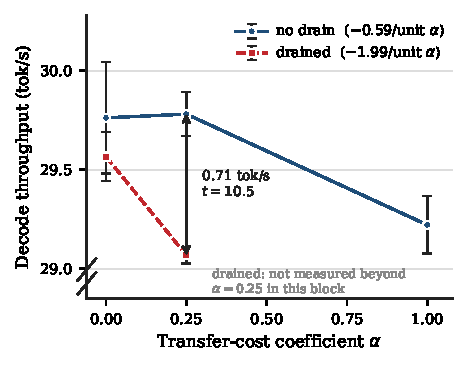
\includegraphics[width=0.62\columnwidth]{fig7_drain}
  \caption{Throughput against the transfer coefficient with and without
  the pipeline drain, from the drain-control block alone. Fitted slopes
  are given in the legend rather than drawn as data. The drained series
  stops at $\alpha = 0.25$ because that is where this block's drained
  data stops; it is not extrapolated, and the cooled sweep's drained
  curve is deliberately not overlaid (see text). The marked contrast at
  $\alpha = 0.25$, the one coefficient measured under both conditions,
  is the finding. The gap between the two series is what draining
  costs; that it opens with $\alpha$ rather than holding constant is
  the interaction quantified in Table~\ref{tab:drain-alpha}. Note the
  truncated ordinate: the whole effect spans $0.7$\,tok/s on a base of
  ${\approx}29.5$.}
  \label{fig:drain}
\end{figure}

\paragraph{Why it matters.} The undrained rows are the finding, and
Figure~\ref{fig:drain} shows the shape. At $\alpha = 0.25$ without
draining, throughput is statistically indistinguishable from
$\alpha = 0$ ($+0.019 \pm 0.174$, $t = 0.11$): at that coefficient the
injected delay is not merely small but undetectable. The absorption is
not unlimited, and we are careful not to overstate it --- by
$\alpha = 1$ the undrained run has lost $0.541 \pm 0.183$\,tok/s
($t = -2.96$), a real $1.8\%$, which is what one expects once the
injected sleep grows to ${\approx}3.1$\,ms against a
${\approx}34$\,ms step. The honest statement is that asynchronous
dispatch \emph{largely absorbs} an undrained delay, not that it hides
it entirely, and the size of the effect is the comparison that matters:
$-0.588$\,tok/s per unit $\alpha$ undrained against $-1.991$ drained,
a factor of $3.4$.

The cleanest single contrast is at $\alpha = 0.25$, the one coefficient
measured under both conditions, where undrained exceeds drained by
$0.713 \pm 0.068$\,tok/s ($t = 10.5$). We rest the finding on that
within-block comparison rather than on the two slopes, and we do not
overlay the cooled sweep's drained curve to extend the drained series:
the two blocks agree on level, $0.30\%$ at the shared $\alpha = 0$, but
their drained slopes differ ($-1.991 \pm 0.300$ against $-1.197 \pm
0.052$, $t = -2.61$), and a shared anchor calibrates level rather than
slope. Splicing them would assert the one property the data declines to
support, and would put a kink at $\alpha = 0.25$ that no reader could
attribute to curvature rather than to the block change. Whether real
curvature exists in the first quarter of the range is unresolved here;
a block running drained points beyond $\alpha = 0.25$ alongside the
undrained ones would settle it.

A simulator that injects a sleep and does not drain therefore measures
far less than it believes. The complementary warning needs stating more
carefully than we first stated it: a simulator that drains is not
paying a fixed instrumentation tax that could be subtracted off
afterwards. The drain's cost is the delay it stops the pipeline
absorbing, so it scales with the very quantity being simulated, and
there is no calibration run at $\alpha = 0$ that would recover it.
What a drained simulator measures is the injected delay under a
dispatch discipline the real system does not have.

The methodological consequence is general. Delay injection is a common
way to model an interconnect one does not have, and on an
asynchronously dispatched accelerator it does not work without a
blocking discipline whose cost must then be measured and subtracted.
Our $\alpha$ curve should be read as the cost of a recall that
\emph{blocks}, which is defensible as a model of discrete memory but is
not the same quantity as $\alpha \cdot \text{bytes}$.

% ---------------------------------------------------------------
\section{Finding 4: Capacity Limits Appear at Execution}
\label{sec:f4}

\paragraph{What we measured.} The largest context the upstream policy
can actually run on this device, probed two ways: by allocation alone,
and with a prompt long enough that the allocated memory is written.

\paragraph{Result.} Allocation is not the binding step. Probing with a
short prompt at $C = 16384 \ldots 131072$, every context loads and
generates --- at $C = 131072$ the runtime reports $4685$\,MiB of model,
$16384$\,MiB of KV, and $8468$\,MiB of compute scratch, a $29537$\,MiB
working set against the advisory $16384$\,MiB, and still returns
successfully. The recommendation is advisory and macOS backs
unified-memory buffers lazily, so a context whose buffers cannot all be
resident nonetheless ``fits''.

\begin{table}[t]
  \centering
  \caption{Where the limit appears; $n = 1$ per configuration, the
  outcome being binary. Same configurations, given a
  16384-token prompt so the memory is touched. Failure is the Metal
  driver refusing the command buffer on the \emph{first} ubatch, not a
  cache-full guard or a length check. Flash attention off.}
  \label{tab:capacity}
  \renewcommand{\arraystretch}{1.25}
  \begin{tabular}{@{}rrrrrl@{}}
    \toprule
    $C$ & \textbf{KV} & \textbf{Scratch} & \textbf{Device} &
      $\times$\textbf{budget} & \textbf{Result} \\
    \midrule
    $32768$  &  $4096$ & $2132$ & $10913$ & $0.67$ & completes \\
    $49152$  &  $6144$ & $3188$ & $14017$ & $0.86$ & completes \\
    $65536$  &  $8192$ & $4244$ & $17121$ & $1.05$ & out of memory \\
    $81920$  & $10240$ & $5300$ & $20225$ & $1.23$ & out of memory \\
    $131072$ & $16384$ & $8468$ & $29537$ & $1.80$ & out of memory \\
    \bottomrule
  \end{tabular}
\end{table}

\begin{figure}[t]
  \centering
  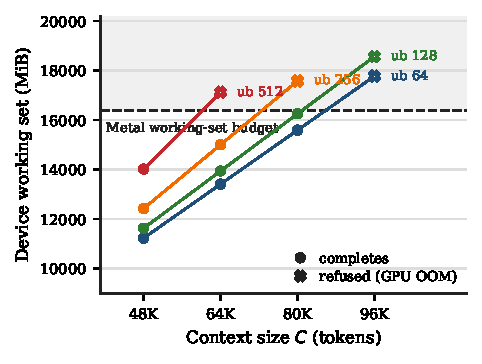
\includegraphics[width=0.62\columnwidth]{fig6_capacity}
  \caption{Device working set against context size for four micro-batch
  settings, with a 16384-token prompt so the memory is written. Filled
  markers complete; crossed markers are refused by the driver. Each
  series crosses the advisory Metal budget (dashed) at a different
  context size, and in every series the transition from completion to
  refusal coincides with that crossing --- the wall sits at the budget,
  and the micro-batch decides which context length reaches it.}
  \label{fig:capacity}
\end{figure}

With the memory touched (Table~\ref{tab:capacity},
Figure~\ref{fig:capacity}), execution fails
with \texttt{kIOGPUCommandBufferCallbackErrorOutOfMemory} as soon as
the working set crosses the advisory budget, between $C = 49152$
($0.86\times$) and $C = 65536$ ($1.05\times$). The correspondence is
tight across the whole sweep: every completing run sits below
$16384$\,MiB, the largest at $0.992\times$, and every refusal above it,
the smallest at $1.045\times$. The largest workable
upstream context on this device lies between those values and is set by
hardware.

\paragraph{A corrected accounting, and the parameter that governs it.}
The device cost of enlarging $C$ is not the $128$\,KiB of KV per token.
With flash attention disabled the attention scratch tensor is
$n_\text{kv} \times n_\text{ubatch} \times n_\text{head}$, so the extra
term is a function of the micro-batch rather than a constant of the
model, and it is \emph{exactly} linear in it: sweeping ubatch
$64 \rightarrow 128 \rightarrow 256 \rightarrow 512$ gives scratch of
$8.29$, $16.57$, $33.16$, and $66.37$\,KiB per context token, ratios of
$2.00$, $2.00$, $2.00$. Total device cost per token therefore ranges
from $136.3$\,KiB at ubatch $64$ to $194.4$\,KiB at ubatch $512$,
approaching the $128$\,KiB of KV alone as the micro-batch shrinks. A
KV-only calculation understates the device cost by between $6\%$ and
$52\%$, and by $52\%$ at the common default of $512$.

The ceiling moves with it, by about $1.7\times$ across the swept range:
the largest workable $C$ goes from $49152$ at ubatch $512$ to $81920$
at ubatch $64$ and $128$. Predicting each ceiling from the measured
per-token cost, as $(16384 - 4685)\,\text{MiB}$ divided by the device
cost per token, gives $61\,600$, $74\,300$, $82\,900$, and $87\,900$
for ubatch $512$ through $64$ --- and each prediction falls inside the
measured bracket. This is the constructive half of the finding: the
arithmetic works, once it counts the right things. What no amount of
arithmetic supplies is the knowledge that the buffers will be refused
at execution rather than at allocation.

The capacity a smaller micro-batch buys appears not to be paid for in
prefill. At $C = 49152$, the one context all four settings run, prefill
throughput on the $16384$-token prompt is $260$, $259$, $268$ and
$237$\,tok/s for ubatch $64$ through $512$: a $3.3\%$ spread with no
monotone trend, and the slowest setting is the \emph{largest}
micro-batch rather than the smallest. At $C = 65536$ the three settings
that run spread by $1.6\%$. We state this as a non-effect at the
available resolution and not as an ordering --- these are single
uncooled runs from a sweep built to find the OOM boundary, and the
spread sits inside the thermal variation we see elsewhere, so the
apparent penalty at ubatch $512$ is not a result. The interpretation we
would offer, untested, is that prefill here is not
parallelism-limited: with the fused kernel off a larger micro-batch
buys wider GEMMs but proportionally more scratch traffic through the
same unified memory, and over this range the two appear to cancel.

One qualifier belongs with the word ``ceiling''. The run closest to the
wall without crossing it, ubatch $128$ at $C = 81920$ and $0.992\times$
the budget, took $251.8$\,s against $62$--$71$\,s for every other
completing run in the sweep --- a $4\times$ slowdown at the same work,
observed once and not repeated. Between roughly $0.99\times$ and
$1.045\times$ the behaviour degrades sharply and then fails outright,
so the transition is not a clean edge. We did not investigate further,
and record it because ``the wall is sharp'' would be too tidy a
description of what we measured.

\paragraph{Why it matters.} Two consequences. For anyone benchmarking
unified memory, allocation success is not evidence of capacity, and a
probe that only allocates will report a limit that does not exist and
miss the one that does. For anyone sizing a cache, the scratch term
must be counted, it is set by a parameter most tuning guides treat as a
throughput knob rather than a capacity one, and it depends on the
kernel: with flash attention enabled the scratch collapses to a
constant $258.5$\,MiB, an $18\times$ reduction, and the ceiling moves
accordingly.

\paragraph{What the ceiling does not buy.} We initially read this
result as a feasibility claim --- that beyond some context length only
a bounded-device policy runs at all --- and it does not survive
measurement. On a $65\,536$-token prompt, two upstream configurations
complete the workload \emph{losslessly}, holding the entire prompt: at
ubatch $64$ with $C = 81920$ and the fused kernel off, and at ubatch
$512$ with $C = 73728$ and the fused kernel on. Both were hidden from
our earlier probing by holding ubatch and the kernel fixed at their
defaults, which is exactly the accounting error this section is about.

\begin{table}[t]
  \centering
  \caption{Completing a $65\,536$-token prompt; $n = 1$ per
  configuration. Exact retention is the
  slowest lossless route, and buys a smaller device working set rather
  than feasibility.}
  \label{tab:65k}
  \renewcommand{\arraystretch}{1.25}
  \begin{tabular}{@{}lrrl@{}}
    \toprule
    \textbf{Configuration} & \textbf{Device MiB} & \textbf{tok/s} &
      \textbf{Lossless?} \\
    \midrule
    Exact retention, $C = 4096$ $+$ host tier & $5481$  & $1.50$  & yes \\
    Rolling window, $C = 4096$                & $5481$  & $27.68$ & no  \\
    H2O, $C = 4096$                           & $5738$  & $31.63$ & no  \\
    Upstream, ubatch $64$, $C = 81920$        & $15588$ & $5.86$  & yes \\
    Upstream fused, ubatch $512$, $C = 73728$ & $14160$ & $15.99$ & yes \\
    \bottomrule
  \end{tabular}
\end{table}

Table~\ref{tab:65k} gives the corrected picture. What exact retention
provides is device footprint at a given context length: it completes
the workload with a $5481$\,MiB working set, $2.8\times$ smaller than
the smallest upstream configuration that also completes it losslessly
and $2.6\times$ smaller than the fastest, and it pays $3.9$--$10.7
\times$ in decode throughput for that. It is a memory-for-throughput
trade, measured in both directions, and not a capability that upstream
lacks.

We state this at length because the error is instructive and we made it
three times in this project. Each time, a claim about what the baseline
\emph{cannot} do turned out to be a claim about a baseline we had
configured badly --- pinned at a default ubatch here, at a fixed kernel
here and elsewhere, at an error-on-overflow policy earlier. A capacity
claim is only as strong as the effort spent configuring the system it
says cannot cope.

\paragraph{The limit transplants.} The execution-time failure was
characterised on the upstream policy, and it reproduces in a
configuration it was not derived from. When the spilled tier of
Section~\ref{sec:f1} is allocated device-visibly it is charged against
the working set in full, and the configuration acquires a ceiling it
does not otherwise have: between $81\,920$ and $90\,112$ spilled cells,
matching the headroom arithmetic to within one step of the sweep, and
failing as a refused command buffer rather than a failed allocation.
The same wall, in a different place, reached by a different mechanism.
Findings that survive transplantation to a configuration they did not
come from are the ones worth believing, and this is the strongest
evidence we have for the section.

The ceiling also completes the trade of Section~\ref{sec:f1}
quantitatively. At its largest working capacity the device-visible
configuration holds $C = 1024$ plus roughly $82\,000$ spilled cells,
about $82\,900$ tokens in total. Upstream with the fused kernel reaches
approximately $91\,000$ with the whole context resident and no spill
machinery at all. In the fast configuration, that is, exact retention
is strictly dominated --- slower \emph{and} shorter-reaching than
simply enlarging the cache. Its capacity advantage exists only in the
CPU-pinned configuration, where the tier is invisible to the working
set and a $16$\,GiB tier runs, and its throughput is competitive only
in the device-visible one. The arithmetic puts the crossover, the
context length beyond which only the CPU-pinned configuration completes
losslessly, at roughly $91\,000$ tokens; we predict it rather than
demonstrate it, because prefill alone at that length extrapolates to
hours.

One contrast with the ubatch sweep is worth a line. There the run
closest to the wall slowed fourfold before failing; here throughput is
flat to the wall ($37.89 \rightarrow 36.73$\,tok/s, $-3\%$) and then
stops. The degradation band belongs to configurations where the
compute scratch grows with the context; a large static buffer does not
behave that way.

% ---------------------------------------------------------------
\section{Finding 5: Context Shift Costs More Than Eviction}
\label{sec:f5}

\paragraph{What we measured.} Decode throughput of all four policies on
a 512-token prompt with a 2048-token decode budget, at two cache
budgets, as five policies $\times$ two budgets $\times$ three trials in a single cooled
randomised block, uninstrumented, flash attention off and verified per
arm.

\begin{table}[t]
  \centering
  \caption{Policy comparison, 512-token prompt and 2048-token decode
  budget, five arms $\times$ two budgets $\times$ three trials in one
  cooled block. The upstream policy halts at cache-full; every
  continuation policy completes. The cost of exactness against the
  strongest of them scales with how much sits in the spilled tier.}
  \label{tab:policy}
  \renewcommand{\arraystretch}{1.25}
  \begin{tabular}{@{}llccr@{}}
    \toprule
    \textbf{Policy} & \textbf{Cache} & \textbf{Tokens} &
      \textbf{Spilled} & \textbf{tok/s} \\
    \midrule
    Upstream (halts)          & $C = 1024$ &  512 &    0 & $43.39$ \\
    Rolling window            & $C = 1024$ & 2048 &    0 & $39.40$ \\
    H2O                       & $C = 1024$ & 2048 & 1535 & $42.42$ \\
    Exact, CPU-pinned         & $C = 1024$ & 2048 & 1535 & $30.24$ \\
    Exact, device-visible     & $C = 1024$ & 2048 & 1535 & $38.07$ \\
    \midrule
    Upstream (halts)          & $C = 2048$ & 1536 &    0 & $41.51$ \\
    Rolling window            & $C = 2048$ & 2048 &    0 & $39.38$ \\
    H2O                       & $C = 2048$ & 2048 &  511 & $40.17$ \\
    Exact, CPU-pinned         & $C = 2048$ & 2048 &  511 & $35.62$ \\
    Exact, device-visible     & $C = 2048$ & 2048 &  511 & $39.64$ \\
    \bottomrule
  \end{tabular}
\end{table}

\paragraph{Result.} In Table~\ref{tab:policy}, H2O is faster than the
rolling window at both budgets, by $7.7\%$ at $C = 1024$ and $2.0\%$ at
$C = 2048$. This is
not the ordering one expects from a policy that computes an importance
signal against one that does not.

The same table locates the cost of exactness. H2O, the strongest
continuation policy here, outruns device-visible exact retention by
$11.4\%$ at $C = 1024$ and by $1.3\%$ at $C = 2048$, both ratios taken
against the retaining arm; at the larger budget exact retention is
nonetheless marginally faster than the rolling window.
The premium scales with the size of the spilled tier --- $1535$ cells
against $511$ --- which is the per-cell term of
Section~\ref{sec:f1} reappearing in end-to-end numbers. Exactness is
not intrinsically expensive; it is expensive in proportion to how much
of the context is not resident.

\paragraph{Why.} The reason is mechanical rather than algorithmic. The
rolling window calls \texttt{seq\_add} on every overflow, re-encoding
rotary position embeddings across the entire cache so that surviving
positions remain contiguous. H2O drops cells outright and touches no
positions, accepting a non-contiguous survivor set that slot allocation
handles cell by cell. On this cache layout the ostensibly cheap
baseline is the more expensive mechanism.

\paragraph{Why it matters.} Context shift is widely used as the
low-cost reference point for ``what happens when the cache fills'',
shipping under that name in this
runtime~\cite{llamacpp_contextshift} and as ContextShift in
KoboldCpp~\cite{koboldcpp_contextshift}. On
this runtime it is not, and a policy comparison that treats it as the
cheap option will misattribute the difference to the competing
policy's overhead. We attribute the cost to the position re-encoding
on the evidence of the code path rather than by isolating it
experimentally --- a build that skipped the re-encode would settle it
and we did not make one --- so the projection should be read
conditionally: where a runtime re-encodes positions on eviction, this
cost should be expected, and whether a given runtime does so is an
implementation choice rather than something inherent to windowed
eviction. We verified it in one.

% ---------------------------------------------------------------
\section{Implications}
\label{sec:implications}

\paragraph{For designers of retention mechanisms.} Where the tier is
read matters more than how large it is, and it matters on both cost
terms. Attending the spilled tier on the accelerator over the same
unified pages removes $69\%$ of the fixed cost and $24.5$--$30.5\%$ of the
per-cell cost (Section~\ref{sec:f1}), so a design that keeps the
retained data addressable by the device is worth substantially more
than one that merely keeps it nearby. But the choice is not free: a
device-visible tier is charged against the working set at capacity, and
the resulting ceiling leaves it with less total reach than simply
enlarging the cache. The two configurations are endpoints of a trade
between device footprint and throughput, and a system that wants both
needs a mechanism neither of ours provides --- device-visible residency
charged at occupancy rather than capacity.

\paragraph{For evaluators of cache policies.} Needle retrieval does not
demonstrate the value of losslessness (Section~\ref{sec:f2}). A
heavy-hitter evictor retrieves the needle, and the generality of that
is bounded by our having tested one: H2O, in our own implementation, at
one needle position. We take it as sufficient to refute
``only lossless retention recovers mid-context facts,'' which is a
claim a single counterexample settles, and not as
establishing how eviction families in general behave. If the property of interest is
reproduction rather than recall, it has to be measured directly, and
token-level comparison against a no-eviction reference is the cheapest
way to do it --- but not at any horizon, and not on any prompt. Our own
first attempt used $32$ tokens of a repetitive filler prompt, which is
short enough and redundant enough that an evictor could agree by
chance; extending it revealed that H2O's divergence is immediate on
prose and delayed on filler, and that the shape of the divergence
differs between them. Two cheap disciplines follow: run past the first
mismatch, since the trace afterwards distinguishes a policy that
collapses into a loop from one that decoheres gradually, and check that
the reference itself is not evicting at the horizon being tested.

\paragraph{For anyone modelling an interconnect they do not have.}
Delay injection on an asynchronously dispatched accelerator measures
almost nothing unless the pipeline is drained, and draining does not
give you a clean measurement either: the drain's own cost is not a
constant but grows with the delay being injected, so it cannot be
calibrated away by a run at zero delay (Section~\ref{sec:f3}). Report
the drained and undrained numbers as two different measurements rather
than one measurement and its correction. If you must have a single
number, say which discipline produced it.

\paragraph{For anyone sizing caches on unified memory.} Allocation
success is not capacity, and the binding limit is at execution. The
per-token device cost includes an attention scratch term that is linear
in the micro-batch and collapses under a fused kernel, so the largest
workable context is set by two parameters normally tuned for
throughput. Anyone reporting a capacity limit should report the ubatch
and kernel it was measured at; ours moves by $1.7\times$ across an
ordinary range of the former (Section~\ref{sec:f4}).

\paragraph{On when exact retention is worth its price.} We decline a
universal answer. Where output is consumed by a human reader,
recovering the fact is very likely enough and H2O is the better policy
on this evidence. Where the decode must be reproducible --- evaluation
harnesses, differential testing across builds or quantisations, agentic
pipelines that replay a trajectory and require it to be the same
trajectory --- token-identity is the property being bought, and no
importance heuristic supplies it at any budget. The evidential base for
that recommendation is $512$ generated tokens on two prompts of
differing entropy, at one budget, on one model
(Table~\ref{tab:horizon}); over that horizon retention is identical and
H2O diverges within the first $16$ tokens on both. Exact retention is
exact by construction --- the spilled entries are recalled, not
approximated --- so we know of no mechanism that would break at token
$513$, but the measurement stops where it stops. This paper prices the
property on one implementation; it does not argue that everyone should
pay it.

% ---------------------------------------------------------------
\section{Threats to Validity}
\label{sec:threats}

\paragraph{Single platform, model, and runtime.} All measurements use
one M4~Pro, one quantisation of one 8B model, and one inference
runtime. The scratch coefficient behind Section~\ref{sec:f4} depends on
the head and KV layout, so the KiB-per-token figures are
model-specific; the linearity in ubatch is not. Ceilings there are
bracketed rather than bisected, since the sweep steps $C$ coarsely, and
we report the scaling rather than a specific token count. The prefill
cost of a smaller micro-batch is reported as a non-effect at our
resolution rather than as an absence: single uncooled runs cannot
resolve a few percent, and we have not run a cooled ubatch block,
so a small penalty would be invisible to us. The
mechanisms behind Findings 1, 3, and 5 are properties of the runtime
and the dispatch model rather than of the specific chip, and we expect
them to transfer; we have not verified that they do.

\paragraph{Which layer each finding belongs to.} Finding 1's fixed term
is a property of \emph{our} implementation, not of exact retention as
a concept. Finding 3 is a property of asynchronous dispatch, which is
general. Finding 4 mixes a hardware limit with a runtime accounting
detail. Finding 5 is a property of the position representation in this
runtime. Finding 2 is the most general, being about what a probe can
distinguish.

The same question applies to the coherent-interconnect machines we
raised in Section~\ref{sec:intro} and did not measure. Findings 2 and 3
should carry unchanged: one is about what a retrieval probe can
distinguish between policies, the other about asynchronous dispatch,
and neither depends on where the bytes live. Finding 1's structure
should carry --- a fixed cost for leaving the fused attention path is
not a property of the memory topology --- but its coefficients should
not: a tier reached over NVLink-C2C pays a genuine per-byte transfer,
so we would expect the per-cell term to grow and the fixed term to
matter relatively less, which is the opposite of the balance we
report. Findings 4 and 5 are tied to this runtime's allocator
accounting and position representation and would need re-measuring
outright. The single sentence we would not port is the one that
motivated the work: on a shared pool, demotion moves no bytes. Across
an interconnect it moves them faster than PCIe, which is a different
claim and licenses a different design.

\paragraph{Statistical power and reporting.} Three trials per arm for
the policy comparison, the drain control and the isochronal blocks; a
single run per arm for the passkey probe, the token-identity block and
every capacity outcome, where the result is binary or exactly
reproducible under greedy decoding. Table~\ref{tab:capacity}'s degradation
observation rests on one run and is not repeated. We report a
regression rather than pairwise tests for the
$\alpha$ sweep precisely because the pairwise comparisons do not
support the weight they were originally given. Several quantities are quoted to more digits than the
measurement resolves; we have kept the digits where they are needed to
reproduce a derived value and rounded elsewhere.

\paragraph{Evidence horizon for token-identity.} The claim that
carries the paper's one positive recommendation is established over
$512$ generated tokens on two prompts, at a single budget, on one model
and one quantisation. The six-arm survey in Table~\ref{tab:quality},
which includes the window policies and the idle arm, remains at its
32-token horizon and should not be read as extending that far. Two
prompts is two: they differ in entropy and structure, which is the axis
that matters most for reproducing a token stream, but they cover
neither code, nor non-English text, nor multi-turn interaction. Our H2O
is one implementation of the policy, so its divergence indices are ours
and not the family's --- though an evictor that discards state the
reference used could not plausibly be identical to it.

\paragraph{Comparator fidelity.} Our H2O aggregates importance across
heads and layers because the runtime's KV cell is shared by all of
them, making it less selective than the per-head original. The retrieval
comparison uses one probe, one needle position, and H2O's default
budget split, unswept. SnapKV is not implemented, and most of the
systems in Table~\ref{tab:families} remain unevaluated.

\paragraph{Residual thermal contamination.} The isochronal design
reduces but does not eliminate self-heating, since larger targets
require longer prefills. The per-cell term is therefore an upper
bound.

\paragraph{A randomisation that did not balance.} The second
drain-control block randomised run order but did not constrain it, and
the draw placed the $\alpha = 1$ conditions early and the $\alpha = 0$
conditions late (mean slots $3.0$ and $5.0$ against $7.3$ and $10.7$).
Condition is thus confounded with position, and the two drain contrasts
run in opposite directions with respect to it, which is precisely how a
thermal drift could manufacture the interaction we report. Three checks
say it did not. Residual throughput regressed on slot gives
$+0.0009$\,tok/s per slot ($t = 0.05$), an implied bias of $-0.005$
against a measured interaction of $1.059$; strictly local
adjacent-slot contrasts, immune to any monotone drift, give $+1.027$;
detrended cell means give $+1.064$. We report the defect because
randomisation alone does not guarantee balance at three trials per
cell, and a future block of this kind should balance position
explicitly rather than trusting the draw. Separately, the
$\alpha = 1$ undrained cell is markedly noisier than the other three
($\text{SD}$ $0.428$ against $0.067$--$0.165$) and dominates the
interaction's standard error; using only its coolest slot moves the
estimate to $+0.928$, which changes the third digit and not the
conclusion.

\paragraph{The shape of the drain cost is not measured.} We report the
drain cost at three coefficients and claim only that it is zero at
$\alpha = 0$ and positive beyond it. Four points across two blocks do
not determine how it grows, and because the blocks must not be fitted
jointly we do not fit them.

% ---------------------------------------------------------------
\section{Related Work}
\label{sec:related}

The two policy families of Table~\ref{tab:families} are surveyed above.
Closest to our instrument, Pie~\cite{pie2024} exploits a coherent
high-bandwidth interconnect to swap KV state between GPU and host
during inference, treating low transfer cost as an opportunity;
FastDecode~\cite{he2024fastdecode} migrates the memory-bound part of
decode attention to host CPUs over host-resident KV, which is the
family our policy-3 implementation belongs to. Neither reports the
cost decomposition of Section~\ref{sec:f1}, which is the quantity that
determines whether the approach is cheap.

On the measurement side, our contribution is closer to workload
characterization than to systems design. We are not aware of a study
that reports the drain-versus-delay interaction of
Section~\ref{sec:f3} or the allocation-versus-execution distinction of
Section~\ref{sec:f4} for unified-memory accelerators, both of which we
encountered as errors before recognising them as findings.

% ---------------------------------------------------------------
\section{Conclusion}
\label{sec:conclusion}

Unified memory removes the explicit transfer that KV-cache offloading
systems are built around, and it is tempting to conclude that a cache
on such hardware should never discard anything. We built that policy
and measured it, and the conclusion does not follow. The cost that
remains after the transfer is gone is a fixed per-step price for
leaving the accelerator's fused attention path, not a price proportional
to what is retained --- which means the interesting engineering target
is the handoff rather than the data. And exactness buys less than
expected: a heavy-hitter evictor recovers the same mid-context fact more
cheaply, and what lossless retention uniquely provides is reproduction
of the computation rather than recovery of its inputs.

The methodological findings may outlast the policy ones. Delay
injection without a blocking discipline measures nothing on an
asynchronously dispatched device, and adding the blocking discipline
does not repair it, because the block costs what it exposes rather than
a fixed amount one could subtract; allocation success is not evidence
of capacity on a lazily backed unified pool; and on a passively cooled
accelerator, sweeping a variable in order will produce a trend whether
or not one exists. Each of these reached us as a correction to a
result we had already written down, which is the argument for
publishing the instrument alongside the measurements.

% ---------------------------------------------------------------
\bibliographystyle{ACM-Reference-Format}

\begin{thebibliography}{99}

\bibitem{kwon2023vllm}
W. Kwon, Z. Li, S. Zhuang, Y. Sheng, L. Zheng, C. H. Yu, J. E. Gonzalez,
H. Zhang, and I. Stoica, ``Efficient memory management for large language
model serving with PagedAttention,'' in \emph{Proc. 29th ACM Symp. Operating
Systems Principles (SOSP)}, 2023, pp. 611--626.

\bibitem{zhang2023h2o}
Z. Zhang, Y. Sheng, T. Zhou, T. Chen, L. Zheng, R. Cai, Z. Song, Y. Tian,
C. R\'e, C. Barrett, Z. Wang, and B. Chen, ``H\textsubscript{2}O: Heavy-hitter
oracle for efficient generative inference of large language models,'' in
\emph{Advances in Neural Information Processing Systems}, vol.~36, 2023.

\bibitem{liu2023scissorhands}
Z. Liu, A. Desai, F. Liao, W. Wang, V. Xie, Z. Xu, A. Kyrillidis, and
A. Shrivastava, ``Scissorhands: Exploiting the persistence of importance
hypothesis for LLM KV cache compression at test time,'' in \emph{Advances in
Neural Information Processing Systems}, vol.~36, 2023.

\bibitem{li2024snapkv}
Y. Li, Y. Huang, B. Yang, B. Venkitesh, A. Locatelli, H. Ye, T. Cai, P. Lewis,
and D. Chen, ``SnapKV: LLM knows what you are looking for before generation,''
in \emph{Advances in Neural Information Processing Systems}, vol.~37, 2024.

\bibitem{chen2024nacl}
Y. Chen, G. Wang, J. Shang, S. Cui, Z. Zhang, T. Liu, S. Wang, Y. Sun, D. Yu,
and H. Wu, ``NACL: A general and effective KV cache eviction framework for LLM
at inference time,'' in \emph{Proc. 62nd Annu. Meeting Assoc. Comput.
Linguistics (ACL)}, 2024, pp. 7913--7926.

\bibitem{feng2025adakv}
Y. Feng, J. Lv, Y. Cao, X. Xie, and S. K. Zhou, ``Ada-KV: Optimizing KV cache
eviction by adaptive budget allocation for efficient LLM inference,'' in
\emph{Advances in Neural Information Processing Systems}, vol.~38, 2025.

\bibitem{xiao2024streamingllm}
G. Xiao, Y. Tian, B. Chen, S. Han, and M. Lewis, ``Efficient streaming language
models with attention sinks,'' in \emph{Proc. Int. Conf. Learning
Representations (ICLR)}, 2024.

\bibitem{sheng2023flexgen}
Y. Sheng, L. Zheng, B. Yuan, Z. Li, M. Ryabinin, B. Chen, P. Liang, C. R\'e,
I. Stoica, and C. Zhang, ``FlexGen: High-throughput generative inference of
large language models with a single GPU,'' in \emph{Proc. Int. Conf. Machine
Learning (ICML)}, 2023, pp. 31094--31116.

\bibitem{lee2024infinigen}
W. Lee, J. Lee, J. Seo, and J. Sim, ``InfiniGen: Efficient generative inference
of large language models with dynamic KV cache management,'' in \emph{Proc.
18th USENIX Symp. Operating Systems Design and Implementation (OSDI)}, 2024,
pp. 155--172.

\bibitem{sun2025shadowkv}
H. Sun, L.-W. Chang, W. Bao, S. Zheng, N. Zheng, X. Liu, H. Dong, Y. Chi, and
B. Chen, ``ShadowKV: KV cache in shadows for high-throughput long-context LLM
inference,'' in \emph{Proc. Int. Conf. Machine Learning (ICML)}, 2025.

\bibitem{cheng2025lmcache}
Y. Cheng, Y. Liu, J. Yao, Y. An, X. Chen, S. Feng, Y. Huang, S. Shen, K. Du,
and J. Jiang, ``LMCache: An efficient KV cache layer for enterprise-scale LLM
inference,'' \emph{arXiv preprint arXiv:2510.09665}, 2025.

\bibitem{he2024fastdecode}
J. He and J. Zhai, ``FastDecode: High-throughput GPU-efficient LLM serving
using heterogeneous pipelines,'' \emph{arXiv preprint arXiv:2403.11421},
2024.

\bibitem{pie2024}
Y. Xu, Z. Mao, X. Mo, S. Liu, and I. Stoica, ``Pie: Pooling CPU memory
for LLM inference,'' \emph{arXiv preprint arXiv:2411.09317}, 2024.

\bibitem{llamacpp_contextshift}
ggml-org, ``\texttt{llama.cpp},'' GitHub repository, context-shift feature
(\texttt{-{}-context-shift}). [Online]. Available:
\url{https://github.com/ggml-org/llama.cpp}

\bibitem{koboldcpp_contextshift}
LostRuins (Concedo), ``KoboldCpp,'' GitHub repository, ContextShift
feature. [Online]. Available:
\url{https://github.com/LostRuins/koboldcpp}

\bibitem{mlx2024}
Apple Inc., ``Unified memory,'' MLX Documentation, 2024. [Online]. Available:
\url{https://ml-explore.github.io/mlx/build/html/usage/unified_memory.html}

\bibitem{apple2024m4pro}
Apple Inc., ``Apple M4 Pro chip specifications,'' 2024. [Online]. Available:
\url{https://support.apple.com/en-us/111893}

\bibitem{nvidia2024gh200}
NVIDIA Corporation, ``NVIDIA Grace Hopper Superchip architecture,'' 2024.
[Online]. Available:
\url{https://www.nvidia.com/en-us/data-center/grace-hopper-superchip/}

\end{thebibliography}

% ---------------------------------------------------------------
\appendix
\section{Artifact and Traceability}
\label{sec:artifact}

The fork, the harnesses, the raw result files and the per-experiment
analyses are archived together. Every quantitative claim in this paper
resolves through Table~\ref{tab:trace} to the harness that produced the
data, the file the data lives in, and an analysis file that states the
protocol, the exclusions and the arithmetic. The analyses were written
at the time of each run rather than reconstructed afterwards, so they
also record results that did not survive: superseded blocks are marked
as such in place rather than deleted, and two of them are cited in
Section~\ref{sec:method} as methodological findings.

Reproducing a rate requires the thermal protocol of
Section~\ref{sec:method} and an otherwise idle machine; reproducing a
capacity outcome, a token sequence or a spill count does not, since
those are binary or deterministic. The model is not redistributed:
every run uses Llama~3.1~8B~Instruct at Q4\_K\_M, fetched separately.

\begin{table*}[t]
  \centering
  \caption{Traceability. Harnesses are under \texttt{scripts/}, result
  files under the directory named, and analyses under
  \texttt{artifacts/}. Where a claim was corrected after first being
  published in an analysis file, the correcting file is listed second.}
  \label{tab:trace}
  \renewcommand{\arraystretch}{1.2}
  \footnotesize
  \begin{tabular}{@{}p{0.20\textwidth}p{0.20\textwidth}p{0.26\textwidth}p{0.28\textwidth}@{}}
    \toprule
    \textbf{Claim} & \textbf{Harness} & \textbf{Data} & \textbf{Analysis} \\
    \midrule
    Eq.~(\ref{eq:recall-cost})--(\ref{eq:recall-cost-dev}), $\gamma$,
      $\delta$, Fig.~\ref{fig:recall}
      & \texttt{run\_b2\_cooled.py}, \texttt{make\_fig5\_recall\_cost.py}
      & \texttt{stress\_results/b2\_isochronal\_both\_modes.csv}
      & \texttt{b2\_cooled/B2\_analysis.txt}; fit spec and regressor in
        \texttt{b2\_cooled/REGRESSION\_SPEC.txt} \\
    Isochronal design; the confounded long-run slope
      & \texttt{run\_recall\_cost\_isochronal.py}
      & \texttt{stress\_results/recall\_cost\_isochronal.csv},
        \texttt{recall\_cost\_steps\_A\_p3\_long.csv}
      & \texttt{recall\_cost/recall\_cost\_analysis.txt} \\
    Device-visible tier; counterbalanced A/B failure
      & \texttt{run\_b1\_ceiling.py}, \texttt{run\_b1\_interleaved.py}
      & \texttt{stress\_results/b1\_device\_tier\_ceiling.csv},
        \texttt{b1\_interleaved\_ab.csv}
      & \texttt{b1\_gpu\_tier/B1\_triage.txt},
        \texttt{B1\_verification\_and\_ceiling.txt} \\
    \midrule
    Table~\ref{tab:quality}: retrieval and 32-token continuation
      & \texttt{run\_quality\_arms\_unified.py}
      & \texttt{quality\_results/quality\_arms\_unified.csv}
      & \texttt{quality\_unified/quality\_arms\_analysis.txt} \\
    H2O comparator fidelity
      & \texttt{run\_quality\_probe.py}
      & \texttt{quality\_results/quality\_probe.csv}
      & \texttt{h2o\_comparator/h2o\_analysis.txt} \\
    Table~\ref{tab:horizon}: 512-token identity, two prompts
      & \texttt{run\_token\_horizon.py}
      & \texttt{quality\_results/token\_horizon.csv}, full ID sequences
        in \texttt{token\_horizon/sequences/}
      & \texttt{token\_horizon/token\_horizon\_analysis.txt} \\
    \midrule
    $\alpha$ sweep slope
      & \texttt{run\_alpha\_sweep\_p3.py}
      & \texttt{alpha\_results/p3\_alpha\_sweep\_cooled\_master.csv}
      & \texttt{r2\_policy3/alpha\_sweep\_cooled\_analysis.txt}
        (supersedes \texttt{alpha\_sweep\_analysis.txt}, thermally
        masked) \\
    Table~\ref{tab:drain}, Fig.~\ref{fig:drain}
      & \texttt{run\_drain\_control.py}, \texttt{make\_fig7\_drain.py}
      & \texttt{alpha\_results/p3\_drain\_control\_master.csv}
      & \texttt{drain\_control/drain\_control\_analysis.txt},
        \texttt{fig7\_provenance.txt} \\
    Table~\ref{tab:drain-alpha}: drain$\times\alpha$ interaction;
      withdrawal of the $71/29$ split
      & \texttt{run\_drain\_alpha1.py}
      & \texttt{alpha\_results/p3\_drain\_alpha1\_master.csv}
      & \texttt{drain\_alpha1/drain\_alpha\_interaction\_analysis.txt}
        (supersedes the decomposition in
        \texttt{drain\_control/drain\_control\_analysis.txt}) \\
    \midrule
    Table~\ref{tab:capacity}, Fig.~\ref{fig:capacity}: scratch term,
      ceilings, ubatch linearity, prefill non-effect
      & \texttt{run\_f4\_phaseA.py}, \texttt{make\_fig6\_capacity.py}
      & \texttt{stress\_results/f4\_a1\_ubatch\_sweep.csv}
      & \texttt{f4\_phaseA/F4\_A1\_ubatch\_sweep.txt},
        \texttt{ubatch\_prefill\_tradeoff.txt} \\
    Table~\ref{tab:65k}: upstream completes the workload
      & \texttt{run\_capacity\_workload.py}
      & \texttt{stress\_results/f4\_a2\_continuation\_arms.csv},
        \texttt{f4\_a3\_flash\_attn\_capacity.csv}
      & \texttt{f4\_phaseA/F4\_A2\_continuation\_arms.txt},
        \texttt{F4\_A3\_flash\_attention\_capacity.txt} \\
    Allocation-versus-execution; advisory-budget ratios
      & \texttt{run\_capacity\_probe.py}
      & \texttt{stress\_results/capacity\_probe.csv}
      & \texttt{capacity\_probe/capacity\_analysis.txt}; unit
        correction in \texttt{CORRECTION\_2026-08-07\_budget\_units.txt} \\
    \midrule
    Table~\ref{tab:policy}: policy comparison, exactness premium
      & \texttt{run\_policy\_compare\_cooled.py}
      & \texttt{stress\_results/r3\_policy\_compare\_cooled\_master.csv}
      & \texttt{r3\_policy\_compare/policy\_compare\_analysis.txt} \\
    \bottomrule
  \end{tabular}
\end{table*}

Three entries in Table~\ref{tab:trace} point at more than one analysis
file, and in each case the second corrects the first. We list them that
way deliberately. The $71/29$ decomposition, the advisory-budget ratios
and the isochronal slope were all published internally before they were
right, and a table that showed only the surviving file would hide the
step that mattered most. Blocks that were superseded outright are
retained under \texttt{stress\_results/SUPERSEDED.md} with the reason.

\end{document}
